\section{Optimization Algorithms}

\subsection{Mini-Batch Gradient Descent}

Training NN with a large data set can be slow. Sometimes memory isn't large enough to fit all data in at once, or using the entire data set for a single iteration of gradient descent would take longer than it's worth. We can split our $m$ training examples into mini-batches of a specified size (usually a power of 2) and small enough that it fits into CPU/GPU. We denoted our mini-batch number by $t = 1, 2, \dots, \lceil \frac{m}{\text{mini-batch size}} \rceil$, and use $X^{\{ t\}}$, $Y^{\{ t\}}$, and $J^{\{ t\}}$ to denote the examples, labels, and cost for mini-batch $t$. One pass through the entire data set is called an epoch. 

\subsection{Batch vs. Mini-Batch vs. Stochastic Gradient Descent}

\begin{multicols}{2}
\begin{itemize}[wide, labelwidth=!, labelindent=0pt]
\itemsep0em 
    \item Stochastic gradient descent has mini-batch size of $1$ (purple). Often too noisy regarding cost minimization and lose speedup from vectorization.
    \item Batch gradient descent has mini-batch size of $m$ (blue). Sometimes too long per iteration. \vspace*{-\baselineskip}
\end{itemize}
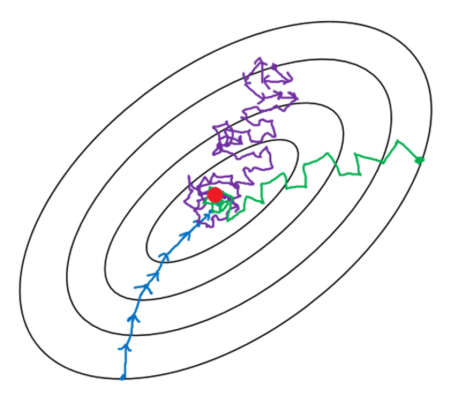
\includegraphics[width=2.3cm]{images/mini_batch_sizes.png}
\end{multicols}

\begin{itemize}[wide, labelwidth=!, labelindent=0pt]
\itemsep0em 
    \item Mini-batch gradient descent has mini-batch size in $(1,m)$ (green). Faster learning while maintaining some advantage from vectorization. Doesn't always converge, but can reduce learning rate when getting close. \vspace*{-\baselineskip}
\end{itemize}

\subsection{Exponentially Weighted Averages}

We calculate exponentially weighted averages across time points $t$ where $v_0 = 0$ and $v_t = \beta v_{t-1} + (1 - \beta) \theta (t)$. Then, $v_t$ is the average over approximately the last $\frac{1}{1 - \beta}$ time points. If we want an average over time points, then exponentially weighted averages are better than sliding window averages because they require less memory. However, starting with $v_0 = 0$ biases our average. To correct for this, we divide our calculation of $v_t$ by $1 - \beta ^t$ yielding $v_t = \frac {\beta v_{t-1} + (1 - \beta) \theta (t)}{1 - \beta ^t}$.

\subsection{Gradient Descent with Momentum}

Momentum helps the cost function to go to the minimum point in a more fast and consistent way.

$V_{dW} = \beta * V_{dW} + (1 - \beta) dW$

$V_{db} = \beta * V_{db} + (1 - \beta) db$

$W := W - \alpha V_{dW}$

$b := b - \alpha V_{db}$

In practice, don't use bias correction because it's resolved in $\approx 10$ iterations. Usually use $\beta = 0.9$.

\subsection{RMSprop}

Also helps the cost function to go to the minimum point in a more fast and consistent way. With RMSprop you can increase your learning rate.

$S_{dW} = \beta_2 * V_{dW} + (1 - \beta_2) (dW * dW)$

$S_{db} = \beta_2 * V_{db} + (1 - \beta_2) (db * db)$

$W := W - \alpha \frac{dW}{\sqrt{S_{dW} + \epsilon}}$ where $epsilon = 10^{-8}$

$b := b - \alpha \frac{db}{\sqrt{S_{db} + \epsilon}}$ where $epsilon = 10^{-8}$

\subsection{Adam Optimizer}

Adaptive Moment Estimation combined ideas from momentum and RMSprop. It tends to work very well.

$V_{dW} = \beta * V_{dW} + (1 - \beta_1) dW$

$V_{dW}^{cor} = \frac{V_{dW}}{1 - \beta_1 ^t}$

$V_{db} = \beta * V_{db} + (1 - \beta_1) db$

$V_{db}^{cor} = \frac{V_{db}}{1 - \beta_1 ^t}$ 

$S_{dW} = \beta_2 * V_{dW} + (1 - \beta_2) (dW * dW)$ 

$S_{dW}^{cor} = \frac{S_{dW}}{1 - \beta_2 ^t}$

$S_{db} = \beta_2 * V_{db} + (1 - \beta_2) (db * db)$

$S_{db}^{cor} = \frac{S_{db}}{1 - \beta_2 ^t}$ 

$W := W - \alpha \frac{V_{db}^{cor}}{\sqrt{S_{dW}^{cor} + \epsilon}}$ where $epsilon = 10^{-8}$

$b := b - \alpha \frac{V_{db}^{cor}}{\sqrt{S_{db}^{cor} + \epsilon}}$ where $epsilon = 10^{-8}$

Hyperparameters usually $\beta_1 = 0.9$, $\beta_2 = 0.999$, $\epsilon = 10^{-8}$, and $\alpha$ needs to be tuned.

\subsection{Learning Rate Decay}

Idea is to slowly reduce learning rate across iterations so the oscillations near the optimum are smaller. Some techniques that are applied across epochs are:

\begin{itemize}[wide, labelwidth=!, labelindent=0pt]
\itemsep0em 
    \item $\alpha = \frac{\alpha_0}{1 + \text{decay\_rate} * \text{epoch\_num}}$
    \item $\alpha = 0.95^{\text{epoch\_num}}\alpha_0$
    \item $\alpha = \frac{k}{\sqrt{\text{epoch\_num}}}\alpha_0$ or $\alpha = \frac{k}{\sqrt{\text{k}}}\alpha_0$ 
    \item Discretely halving $\alpha$ at end of each epoch \vspace*{-\baselineskip}
    \item Manual decay only if training a small number of models
\end{itemize}

\subsection{Problem of Local Optima}

The normal local optima is not likely to appear in a deep neural network because data is usually high dimensional. For point to be a local optima it has to be a local optima for each of the dimensions which is highly unlikely. It is much more likely to get to the saddle point. Sometimes plateaus can make learning slow when gradient is close to zero for a long time, but small random perturbations can help along with algorithms like momentum, RMSprop or Adam.

